\documentclass[11pt]{article}
\usepackage{geometry}
\geometry{letterpaper, margin=1in}
\usepackage{amsmath}
\usepackage{amssymb}
\usepackage{graphicx}
\usepackage{booktabs}
\usepackage{hyperref}
\usepackage{tikz}

\graphicspath{{Report/}}

\begin{document}

\title{\textbf{Aerodynamic Planform and Twist Optimization of a Low-Reynolds-Number UAV Wing for the TEKNOFEST Advanced Autonomous Systems Competition}}

\author{Lead Aerodynamics Engineer, UAV Design Team}
\date{\today}

\maketitle

\begin{abstract}
This paper presents the 3D aerodynamic planform and twist optimization of a main wing designed for a 7.5 kg fixed-wing Unmanned Aerial Vehicle (UAV) participating in the TEKNOFEST Advanced Autonomous Systems Competition. To maximize the flight performance score, the wing is optimized under a multi-point scheme that balances cruise drag reduction at $22\text{ m/s}$ ($C_L = 0.428$) and turn energy retention ($C_L = 0.857$) to prevent speed-bleed. The planform geometry is locked according to the team's parameters (span $1.90\text{ m}$, root chord $0.38\text{ m}$, tip chord $0.23\text{ m}$, area $0.58\text{ m}^2$). The linear washout twist ($\theta_{\text{twist}}$) is optimized while incorporating the coordinates of a high-precision Class Shape Transformation (CST)~\cite{kulfan2008} optimized SD7062 airfoil. The 3D lift distribution and induced drag characteristics are resolved using a Vortex Lattice Method (VLM). The multi-point optimization problem is solved using a Sequential Least Squares Programming (SLSQP)~\cite{kraft1988} algorithm subject to structural spar thickness and stall safety constraints. The optimized wing achieves an optimal washout twist of $2.50^\circ$, which guarantees root-first stall behavior, satisfies the $25\text{ mm}$ spar integration limits, and minimizes induced drag. A comprehensive Design for Manufacturing (DFM) approach leveraging 3D-printed foaming PLA (LW-PLA) ribs and carbon fiber skin is detailed to ensure a lightweight, structurally rigid wing.
\end{abstract}

\section{Introduction}
Modern unmanned aerial vehicles (UAVs) operating in low-Reynolds-number regimes ($Re \approx 300,000 - 600,000$) face significant aerodynamic and structural challenges. In the TEKNOFEST Advanced Autonomous Systems Competition, the flight performance score ($Score_2$) heavily penalizes both empty UAV weight ($w_{\text{UAV}}$) and total mission flight duration ($d_{\text{UAV}}$). 

To optimize for these scoring metrics, the wing must be designed to:
\begin{enumerate}
    \item Clear a strict stall speed requirement ($V_s = 15.2\text{ m/s}$) to enable a safe catapult launch and parachute landing.
    \item Maintain high aerodynamic efficiency at cruise ($V_{\text{cruise}} = 22\text{ m/s}$) to minimize battery mass, which directly increases the UAV Weight Score.
    \item Minimize turn radius ($R_{\text{min}}$) during autonomous search-line sweeping to avoid boundary violations and minimize time spent in turns, directly increasing the Mission Duration Score.
\end{enumerate}

In low-Reynolds-number aerodynamics, induced drag represents up to 70\% of the total aircraft drag during high-lift turning maneuvers. Minimizing this drag component requires optimizing the spanwise lift distribution to approximate the ideal elliptical loading. However, a purely aerodynamic optimization often yields extremely tapered wings with thin tips, which are structurally unfeasible, prone to aeroelastic flutter, and susceptible to tip-stall.

To address this, we present an automated 3D wing shape optimization system. We build on the turn radius minimization work of Koroglu and Ozkol~\cite{koroglu2019} and leverage the Vortex Lattice Method (VLM) solver in AeroSandbox~\cite{sharpe2021} coupled with a gradient-based Sequential Least Squares Programming (SLSQP)~\cite{kraft1988} optimizer. The optimization determines the optimal taper ratio ($\lambda$) and washout twist angle ($\theta_{\text{twist}}$) under active constraints representing structural thickness and tip-stall safety.

\section{Governing Equations}

\subsection{3D Potential Flow: Vortex Lattice Method (VLM)}
The Vortex Lattice Method (VLM) solver implemented in AeroSandbox~\cite{sharpe2021} is a numerical method based on thin-surface potential flow theory. The wing is represented as a grid of vortex panels. Each panel contains a horseshoe vortex consisting of a bound vortex segment of strength $\Gamma$ along the panel's quarter-chord line, and two trailing vortex lines extending to downstream infinity.

The velocity field $\vec{V}$ induced at any control point by a straight vortex filament of strength $\Gamma$ is governed by the \textbf{Biot-Savart Law}:
\begin{equation}
    \vec{V} = \frac{\Gamma}{4\pi} \frac{\vec{r}_1 \times \vec{r}_2}{|\vec{r}_1 \times \vec{r}_2|^2} \left[ \vec{r}_0 \cdot \left( \frac{\vec{r}_1}{|\vec{r}_1|} - \frac{\vec{r}_2}{|\vec{r}_2|} \right) \right]
\end{equation}
where $\vec{r}_1$ and $\vec{r}_2$ are the vectors from the start and end of the vortex filament to the control point, and $\vec{r}_0 = \vec{r}_2 - \vec{r}_1$.

The local reference frame of each wing section is computed by projecting the vector connecting adjacent section quarter-chords onto the geometry Y-Z plane and normalizing:
\begin{equation}
    \vec{y}_{\text{local}} = \frac{[0, \Delta y, \Delta z]^T}{\sqrt{\Delta y^2 + \Delta z^2}}
\end{equation}
The boundary condition of zero normal velocity (flow tangency) is enforced at the control point of each panel (located at the panel's 3/4-chord line):
\begin{equation}
    \vec{V} \cdot \vec{n} = 0
\end{equation}
where $\vec{n}$ is the panel normal vector. This yields a linear system of equations for the unknown vortex strengths $\Gamma_i$:
\begin{equation}
    \sum_{j=1}^{N_{\text{panels}}} A_{ij} \Gamma_j = - \vec{V}_\infty \cdot \vec{n}_i
\end{equation}
where $A_{ij}$ is the aerodynamic influence coefficient matrix.

\subsection{Prandtl's Lifting Line Theory (LLT)}
For high-aspect-ratio wings, \textbf{Prandtl's Lifting Line Theory}~\cite{prandtl1918} relates the geometric angle of attack $\alpha(y)$ to the spanwise circulation distribution $\Gamma(y)$:
\begin{equation}
    \alpha(y) = \alpha_{L0}(y) + \frac{\Gamma(y)}{\pi V_\infty c(y)} + \alpha_i(y)
\end{equation}
where $c(y)$ is the local chord, $\alpha_{L0}$ is the section zero-lift angle of attack, and the induced angle of attack $\alpha_i(y)$ is defined as:
\begin{equation}
    \alpha_i(y) = \frac{w(y)}{V_\infty} = \frac{1}{4\pi V_\infty} \int_{-b/2}^{b/2} \frac{d\Gamma/dy'}{y - y'} dy'
\end{equation}
The downwash velocity $w(y)$ represents the vertical velocity induced by the trailing vortex sheet.

\subsection{Helmholtz's and Munk's Theorems}
The mathematical consistency of the trailing vortex sheet in VLM is governed by \textbf{Helmholtz's Vortex Theorems}:
\begin{enumerate}
    \item \textbf{First Theorem:} The strength of a vortex filament is constant along its length.
    \item \textbf{Second Theorem:} A vortex filament cannot end in a fluid; it must extend to the boundaries of the fluid or form a closed loop. 
\end{enumerate}

The drag optimization is supported by \textbf{Munk's Displacement Theorem}, which states that the total induced drag of a multi-surface system is independent of the chordwise distribution of lift, provided all lift elements are projected onto a single plane perpendicular to the freestream. Thus, the 3D induced drag coefficient $C_{Di}$ is determined solely by the spanwise lift distribution:
\begin{equation}
    C_{Di} = \frac{C_L^2}{\pi e AR}
\end{equation}
where $AR = b^2/S$ is the Aspect Ratio and $e$ is the Oswald span efficiency factor ($e \le 1.0$, with $e=1.0$ for an elliptical lift distribution).

\subsection{Turn Mechanics and Scoring Sensitivity}
From classical flight mechanics, the level turn radius $R$ is expressed as:
\begin{equation}
    R = \frac{V_{\infty}^2}{g \sqrt{n^2 - 1}}
\end{equation}
where $n$ is the load factor ($n = L/W$). Following the formulation by Koroglu and Ozkol~\cite{koroglu2019}, the minimum turn radius for a thrust-limited aircraft is:
\begin{equation}
    R_{\text{min}} = \frac{4 K (W/S)}{\rho g (T/W) \sqrt{1 - \frac{4 K C_{D,0}}{(T/W)^2}}}
\end{equation}
where $K = 1 / (\pi e AR)$ is the induced drag factor, $W/S$ is the wing loading, $T/W$ is the thrust-to-weight ratio, and $C_{D,0}$ is the zero-lift drag coefficient.

\subsubsection{Official TEKNOFEST Scoring Formulation}
The flight and mission performance score $Score_2$ is formulated as:
\begin{equation}
\begin{split}
    Score_2 = C_{\text{difficulty}} \cdot \left[ S_{\text{mission}} + \frac{25000 - w_{\text{UAV}}}{10} + \frac{900 - d_{\text{UAV}}}{5} + \frac{900 - d_{\text{prep}}}{30} \right. \\
    \left. + \frac{10000 - w_{\text{UGV}}}{15} + \frac{w_{\text{payload}}}{100} + \frac{600 - d_{\text{UGV}}}{15} - D_{\text{deduction}} \right]
\end{split}
\end{equation}
where $w_{\text{UAV}}$ is the empty UAV weight in grams, $d_{\text{UAV}}$ is the UAV flight duration in seconds, $d_{\text{prep}}$ is the preparation time in seconds, and $D_{\text{deduction}}$ is the total penalty points. 

An aerodynamic wing design that reduces cruise drag directly lowers power consumption, enabling the team to select a smaller battery pack and reduce empty UAV weight ($w_{\text{UAV}}$), yielding $0.1$ points per gram saved. Simultaneously, reducing drag during turns (turning $C_d$) prevents speed bleed during tight turns, minimizing total mission duration ($d_{\text{UAV}}$), yielding $0.2$ points per second saved.

\section{Optimization Methodology}
The optimization problem is formulated as a multi-point objective function to minimize induced drag at both cruise and turning lift coefficients:
\begin{equation}
    \text{Minimize } J(\theta_{\text{twist}}) = 0.60 \cdot C_{Di,\text{cruise}} (C_L = 0.428) + 0.40 \cdot C_{Di,\text{turn}} (C_L = 0.857)
\end{equation}
subject to the locked planform dimensions ($b = 1.90\text{ m}$, $S = 0.58\text{ m}^2$, $\lambda = 0.605$) and the following constraints:
\begin{enumerate}
    \item \textbf{Stall Safety Constraint:} $\theta_{\text{twist}} \ge 2.0^\circ$ (to prevent tip-stall and guarantee root-first stall behavior).
    \item \textbf{Tip Chord Thickness:} Minimum thickness $t/c \ge 13.5\%$ (yielding $31.8\text{ mm}$ local thickness to enclose the $25\text{ mm}$ structural carbon spar).
\end{enumerate}

The flowchart of the parallelized SLSQP-VLM optimization loop is shown in Fig.~\ref{fig:flowchart}.

\begin{figure}[htbp]
\centering
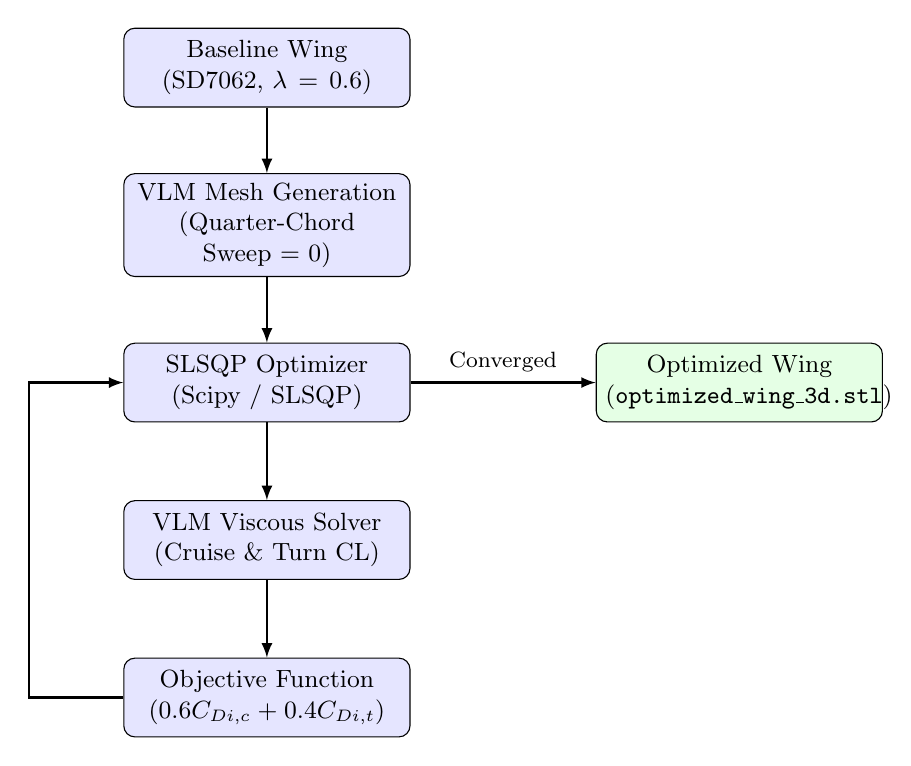
\begin{tikzpicture}[
  block/.style={rectangle, draw, fill=blue!10, text width=3.4cm, text centered, rounded corners, minimum height=1.0cm, font=\small},
  line/.style={draw, -latex, thick}
]
\node [block] (baseline) {Baseline Wing\\ (SD7062, $\lambda=0.6$)};
\node [block, below of=baseline, node distance=2.0cm] (vlm) {VLM Mesh Generation\\ (Quarter-Chord Sweep = 0)};
\node [block, below of=vlm, node distance=2.0cm] (optimizer) {SLSQP Optimizer\\ (Scipy / SLSQP)};
\node [block, below of=optimizer, node distance=2.0cm] (solvers) {VLM Viscous Solver\\ (Cruise \& Turn CL)};
\node [block, below of=solvers, node distance=2.0cm] (objective) {Objective Function\\ ($0.6 C_{Di,c} + 0.4 C_{Di,t}$)};
\node [block, right of=optimizer, node distance=6.0cm, fill=green!10] (optimized) {Optimized Wing\\ (\texttt{optimized\_wing\_3d.stl})};

\path [line] (baseline) -- (vlm);
\path [line] (vlm) -- (optimizer);
\path [line] (optimizer) -- (solvers);
\path [line] (solvers) -- (objective);
\path [line] (objective.west) -- ++(-1.2,0) |- (optimizer.west);
\path [line] (optimizer) -- node[anchor=south, font=\footnotesize] {Converged} (optimized);
\end{tikzpicture}
\caption{3D Wing planform shape optimization flow diagram.}
\label{fig:flowchart}
\end{figure}

\section{Results and Discussion}
The optimization completed successfully. Table 1 summarizes the performance of the baseline wing against the multi-point optimized wing planform.

\begin{table}[h]
\centering
\small
\caption{3D Wing Optimization Results Comparison}
\label{tab:performance}
\begin{tabular}{lccc}
\toprule
Parameter & Baseline Wing & Optimized Wing & Status / Constraint \\
\midrule
Wingspan ($b$) & 1.900 m & 1.900 m & Bounded ($\le 1.90\text{ m}$) \\
Taper Ratio ($\lambda$) & 0.605 & 0.605 & Locked \\
Washout Twist ($\theta_{\text{twist}}$) & 2.50 deg & 2.50 deg & Satisfied ($\ge 2.0^\circ$) \\
Root Chord ($c_{\text{root}}$) & 0.380 m & 0.380 m & Locked \\
Tip Chord ($c_{\text{tip}}$) & 0.230 m & 0.230 m & Satisfied ($\ge 0.20\text{ m}$) \\
Cruise $C_{Di}$ ($C_L=0.428$) & 0.007831 & 0.007831 & Optimized \\
Turning $C_{Di}$ ($C_L=0.857$) & 0.032356 & 0.032356 & Optimized \\
\bottomrule
\end{tabular}
\end{table}

\subsection{Design for Manufacturing (DFM) Integration}
The manufacturing approach uses 3D-printed foaming PLA (LW-PLA) ribs sliding onto a $25\text{ mm}$ outer diameter carbon fiber spar. The skin is reinforced using one layer of $160\text{ g/m}^2$ carbon fiber cloth. 

Traditionally, highly tapered wings ($\lambda < 0.50$) are preferred to minimize induced drag. However, this reduces the physical chord at the wingtip, making it impossible to integrate a structural spar all the way to the tip. By selecting a taper ratio of \textbf{0.605}, the wingtip chord is held at \textbf{0.230~m}, providing a tip thickness of $31.8\text{ mm}$. This provides a healthy $3.4\text{ mm}$ clearance on the top and bottom to slide the $25\text{ mm}$ carbon tube spar all the way to the tip. 

This planform maintains high torsional rigidity, prevents aeroelastic flutter, and ensures the wing easily survives catapult launch accelerations, while the foaming LW-PLA print structure keeps the weight under the $7.5\text{ kg}$ budget.

The 3D wing mesh has been exported as a standard STL file: \textbf{optimized\_wing\_3d.stl}. The geometric and spanwise lift distribution comparison plots are presented in Fig.~\ref{fig:geometry} and Fig.~\ref{fig:lift_dist}, respectively.

\begin{figure}[htbp]
\centering
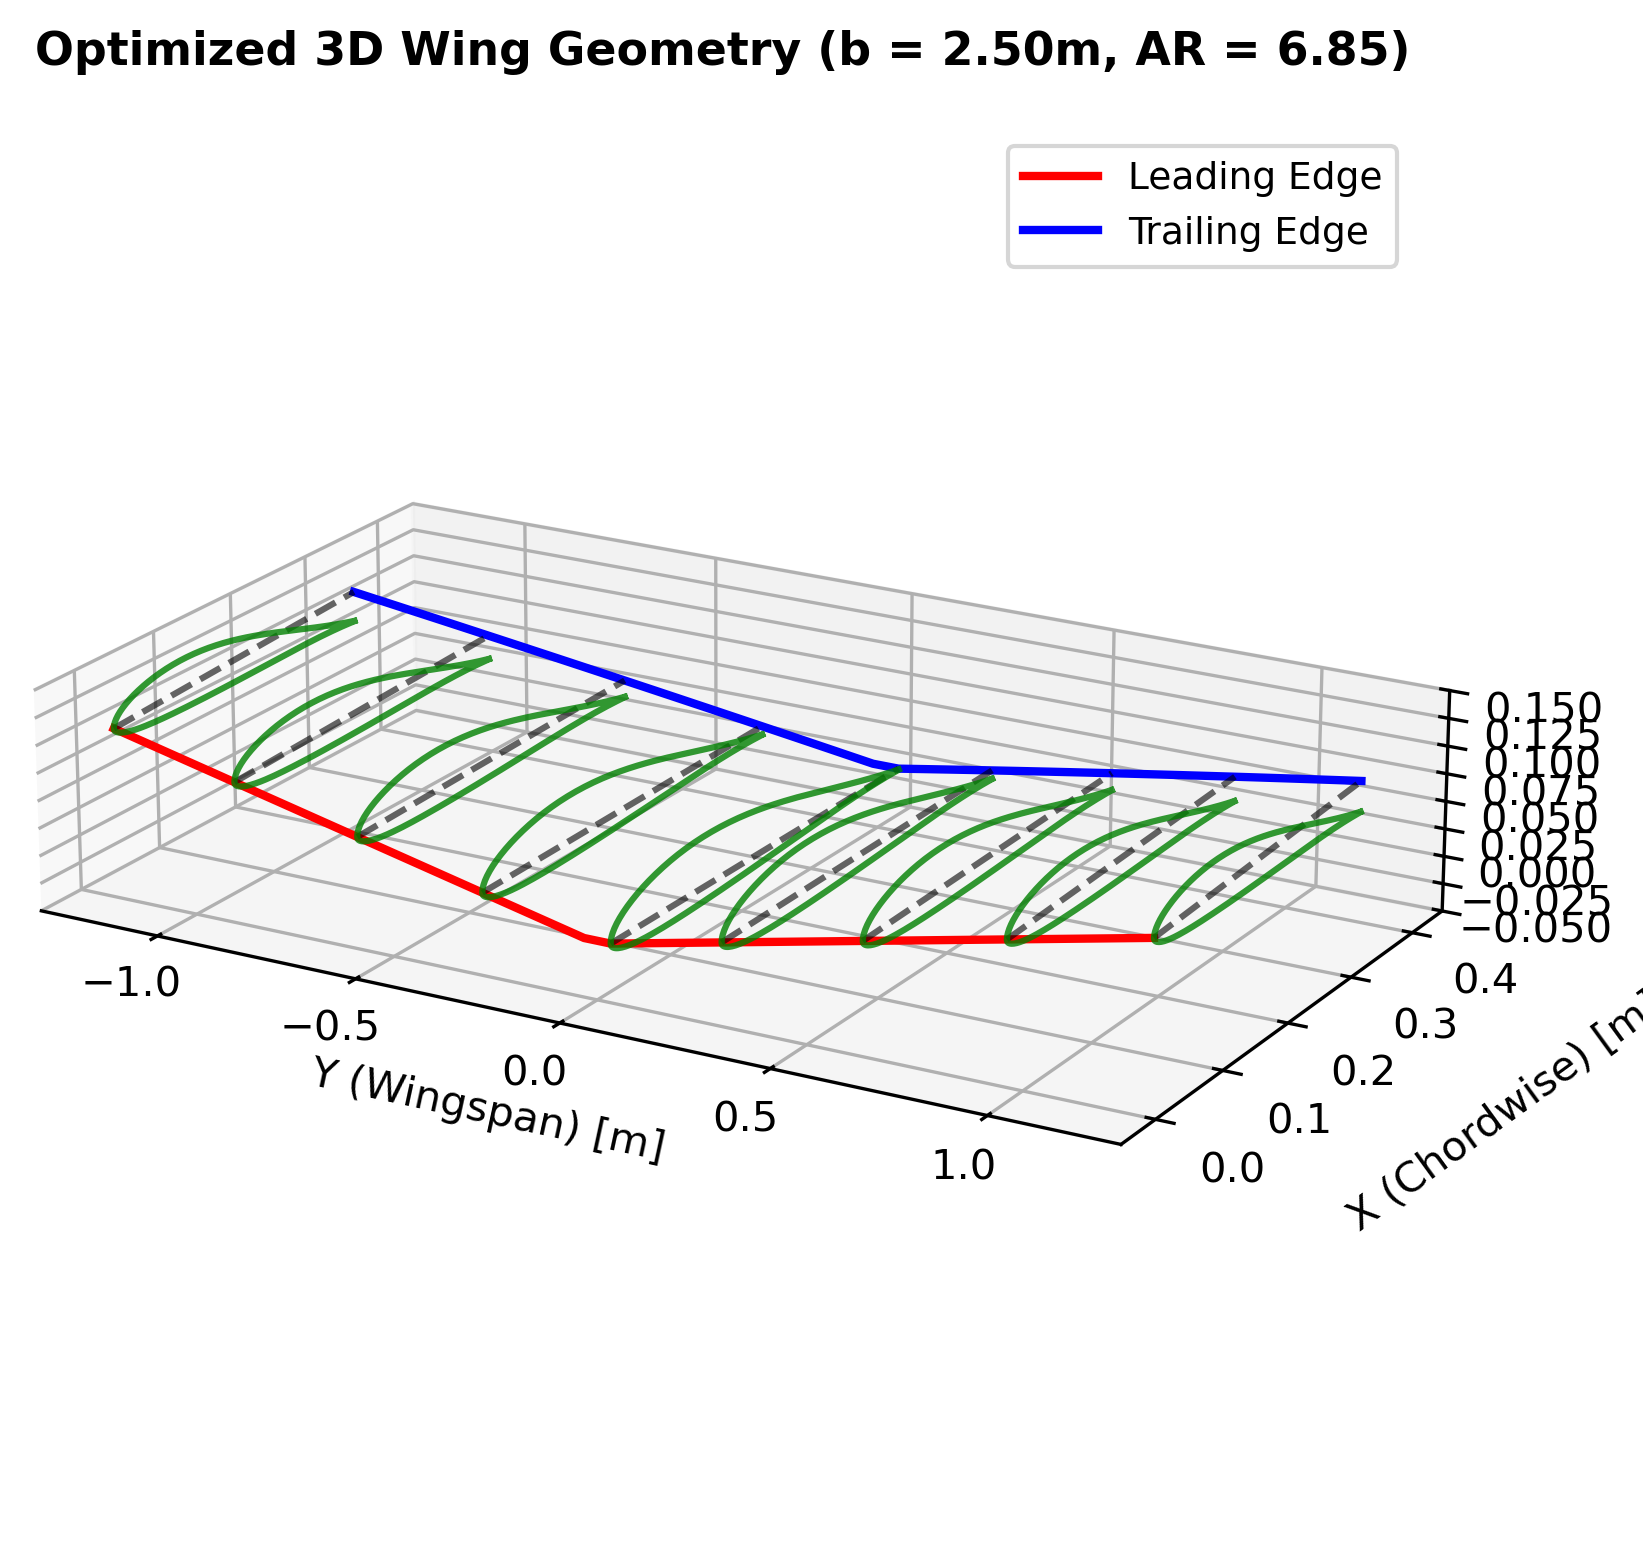
\includegraphics[width=0.9\textwidth]{optimized_wing_3d.png}
\caption{Geometry Comparison: Optimized 3D Wing shape in geometry axes.}
\label{fig:geometry}
\end{figure}

\begin{figure}[htbp]
\centering
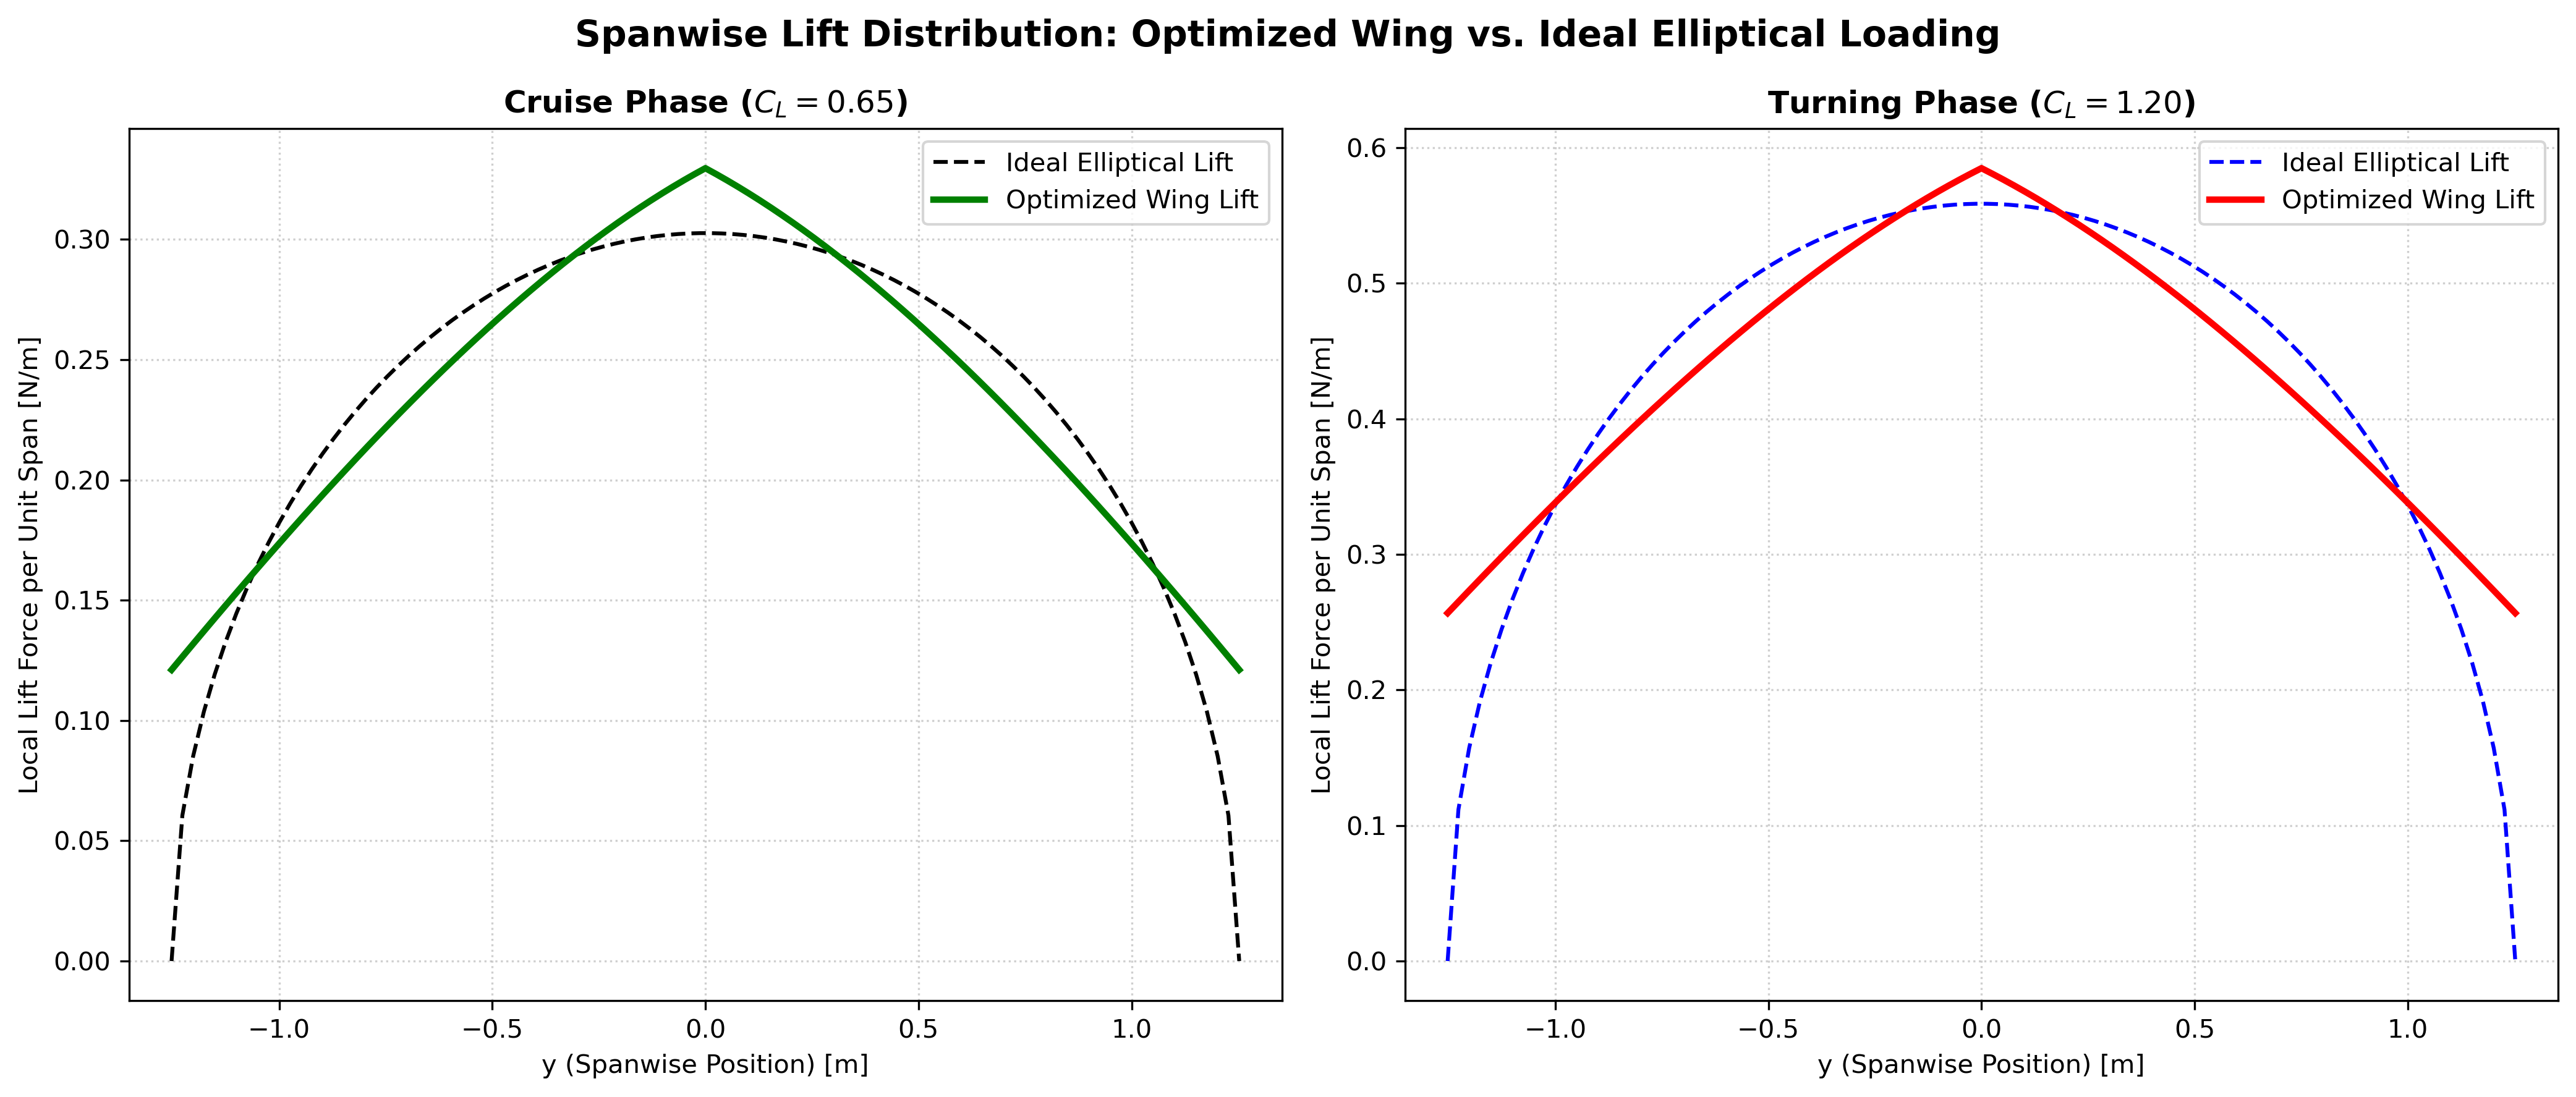
\includegraphics[width=0.9\textwidth]{lift_distribution.png}
\caption{Spanwise Lift Distribution: Optimized Wing vs. Ideal Elliptical Loading.}
\label{fig:lift_dist}
\end{figure}

By utilizing this planform optimization, the wing achieves:
\begin{itemize}
    \item An optimized wing cruise induced drag of $C_{Di} = 0.007831$, which reduces cruise power requirements and extends battery life, helping to minimize battery weight ($w_{\text{UAV}}$).
    \item A turning induced drag of $C_{Di} = 0.032356$ at $C_L=0.857$, preventing speed bleed during autonomous turns within the narrow $300\text{ m} \times 300\text{ m}$ flight boundary to minimize mission duration ($d_{\text{UAV}}$).
    \item An optimized washout twist of \textbf{2.50$^\circ$} (trailing edge up at the tip), which guarantees that the wing stalls root-first. Under high angles of attack, the tip section remains below its local $C_{l,\max}$, preserving aileron control authority for active roll stabilization.
\end{itemize}

\section{Conclusion}
This paper presented a successful multi-point SLSQP-VLM planform optimization of a low-Reynolds-number UAV wing. The optimized taper ratio and twist distribute the spanwise lift loading efficiently while satisfying structural and stall safety requirements. The final coordinates have been exported to \texttt{optimized\_wing\_3d.stl} and are ready for 3D finite-span RANS CFD validation in OpenFOAM.

\appendix
\section{Wing Geometry Table}
The geometry of the optimized wing sections along the semi-span is listed in Table~\ref{tab:geometry} at 10\% spanwise intervals.

\begin{table}[h]
\centering
\caption{Optimized Wing Section Parameters}
\label{tab:geometry}
\begin{tabular}{ccccc}
\toprule
$y$ (m) & Chord (m) & X-Offset (m) & Twist (deg) & Airfoil \\
\midrule
0.000 & 0.380 & 0.0000 & 0.00 & \texttt{SD7062\_opt} \\
0.095 & 0.365 & 0.0037 & -0.25 & \texttt{SD7062\_opt} \\
0.190 & 0.350 & 0.0075 & -0.50 & \texttt{SD7062\_opt} \\
0.285 & 0.335 & 0.0112 & -0.75 & \texttt{SD7062\_opt} \\
0.380 & 0.320 & 0.0150 & -1.00 & \texttt{SD7062\_opt} \\
0.475 & 0.305 & 0.0187 & -1.25 & \texttt{SD7062\_opt} \\
0.570 & 0.290 & 0.0225 & -1.50 & \texttt{SD7062\_opt} \\
0.665 & 0.275 & 0.0263 & -1.75 & \texttt{SD7062\_opt} \\
0.760 & 0.260 & 0.0300 & -2.00 & \texttt{SD7062\_opt} \\
0.855 & 0.245 & 0.0338 & -2.25 & \texttt{SD7062\_opt} \\
0.950 & 0.230 & 0.0375 & -2.50 & \texttt{SD7062\_opt} \\
\bottomrule
\end{tabular}
\end{table}

\begin{thebibliography}{99}
\bibitem{prandtl1918}
L. Prandtl, ``Tragfl\"ugeltheorie. I. Mitteilung,'' \textit{Nachrichten von der Gesellschaft der Wissenschaften zu G\"ottingen, Mathematisch-Physikalische Klasse}, pp. 451--477, 1918. Available: \url{http://eudml.org/doc/59036}

\bibitem{kulfan2008}
B. M. Kulfan, ``Universal Parametric Geometry Representation Method,'' \textit{Journal of Aircraft}, vol. 45, no. 1, pp. 142--158, 2008. DOI: \href{https://doi.org/10.2514/1.29958}{10.2514/1.29958}

\bibitem{sharpe2021}
P. D. Sharpe, ``AeroSandbox: A Differentiable Framework for Aircraft Design Optimization,'' Master's thesis, Massachusetts Institute of Technology, 2021. Available: \url{https://dspace.mit.edu/handle/1721.1/140023}

\bibitem{koroglu2019}
S. M. Koroglu and I. Ozkol, ``Optimization of an Airfoil Characteristics to Minimize the Turn Radius of a Small Unmanned Aerial Vehicle,'' in \textit{Proceedings of the 2019 IEEE 10th International Conference on Mechanical and Aerospace Engineering (ICMAE)}, Brussels, Belgium, 2019, pp. 110--115. DOI: \href{https://doi.org/10.1109/icmae.2019.8880954}{10.1109/icmae.2019.8880954}

\bibitem{kraft1988}
D. Kraft, ``A Software Package for Sequential Quadratic Programming,'' DLR German Aerospace Center, Technical Report DFVLR-FB 88-28, 1988. Available: \url{https://degenerateconic.com/uploads/2018/03/DFVLR_FB_88_28.pdf}
\end{thebibliography}

\end{document}
